% Provenance (never printed): sources/book2/BRIEFS.md, g11-07. Rival and excludable goods, free riding and how public
% goods get provided, the open-access fishery, and the answers with their record. Real numbers:
% figdata/grade-11/07-public-goods-and-commons/ (WDI capture fisheries production for Peru, Iceland and New Zealand; the
% quota dates as a cited table). Ledger: anchoveta and El Nino, the northern cod moratorium, Costello et al. 2008 (via a
% press release), the quota dates, the lighthouse record and its critics, Ostrom 1990 (via reference pages). The WDI series
% is all fish captured by the country, not the anchoveta alone; the reference page's anchoveta tonnages differ from it and
% are not printed. Photograph: Eddystone lighthouse (Commons, PD). The Kestrian fishery is invented.
\chapter{Public Goods and Common Resources}\label{ch:g11:public-goods-and-commons}

In 1970 Peru's fishing fleet landed 12.5 million tonnes of fish, most of it anchoveta, a small fish ground into meal for animal feed.
Three years later it landed 2.3 million. An El Niño had warmed the sea in 1972 and cut the cold, rich water the fish feed in; but the stock had already been reduced
by overfishing. The catch did not pass 12 million tonnes again until 1994.
% figdata: peru_key (1970 12486, 1973 2298, 1994 12001); ledger: g11:anchoveta

No one owned the anchoveta in the sea. Each boat that caught a tonne left one tonne less for the others, and none had a reason to leave fish to breed. This chapter
sorts goods by two questions, whether one person's use leaves less for others and whether anyone can be kept from using them, and shows what goes wrong, and what has
worked, for the goods that markets handle badly.

\begin{openingchart}{Fish caught by Peru's fleet, 1960--2000, in thousands of tonnes a year.}{World Bank, World Development Indicators (capture fisheries production)}
\begin{tikzpicture}
\begin{axis}[omtime, width=0.86\linewidth, height=5.6cm, xmin=1960, xmax=2000, ymin=0, ymax=13500, ylabel={thousand tonnes}, xtick={1960,1965,...,2000},
  y tick label style={/pgf/number format/1000 sep={\,}}, scaled y ticks=false]
\addplot[omDef, thick] table[x=year, y=kt] {figdata/grade-11/07-public-goods-and-commons/out/peru.csv};
\addplot[only marks, mark=*, mark size=1.4pt, omThm] table[x=year, y=kt] {figdata/grade-11/07-public-goods-and-commons/out/peru_key.csv};
\end{axis}
\end{tikzpicture}
\end{openingchart}

\begin{recall}
From the grades 6--9 volume: a property right is the right to use a thing, to keep its fruits and to sell it, protected by law. From
\cref{ch:g11:externalities}: an \omterm{def:g11:externalities:externality}{externality} is an effect on others not paid for through a price. From \cref{ch:g11:oligopoly-and-games}: a \omterm{def:g11:oligopoly-and-games:nash}{Nash equilibrium}, and the
\omterm{def:g11:oligopoly-and-games:prisoners-dilemma}{prisoner's dilemma}, in which each player's best choice leaves both worse off.
\end{recall}

\section{Four kinds of goods}\label{sec:g11:public-goods-and-commons:kinds}

\begin{definition}[Rival and excludable goods]\label{def:g11:public-goods-and-commons:rival}
A good is a \emph{rival good}\index{rival good} when one person's use of it leaves less for others. It is an \emph{excludable good}\index{excludable good}%
\phantomsection\label{def:g11:public-goods-and-commons:excludable} when those who do not pay can be kept from using it.
\end{definition}

\begin{definition}[Private, public and club goods; common resources]\label{def:g11:public-goods-and-commons:private-good}
A \emph{private good}\index{private good} is rival and excludable. A \emph{public good}\index{public good}%
\phantomsection\label{def:g11:public-goods-and-commons:public-good} is neither rival nor excludable. A \emph{club good}\index{club good}%
\phantomsection\label{def:g11:public-goods-and-commons:club-good} is excludable but not rival, at least until it is crowded. A \emph{common resource}\index{common
resource}\phantomsection\label{def:g11:public-goods-and-commons:common-resource} is rival but not excludable.
\end{definition}

\begin{omfigure}
\renewcommand{\arraystretch}{1.5}
\begin{tabular}{l|p{0.36\linewidth}|p{0.36\linewidth}}
 & \textbf{Rival} & \textbf{Not rival} \\ \hline
\textbf{Excludable} & \emph{\omterm{def:g11:public-goods-and-commons:private-good}{private goods}}: bread, a haircut, a bicycle & \emph{\omterm{def:g11:public-goods-and-commons:private-good}{club goods}}: a cinema screening, a streaming service, an uncrowded toll road \\ \hline
\textbf{Not excludable} & \emph{\omterm{def:g11:public-goods-and-commons:private-good}{common resources}}: fish in the open sea, groundwater, a free road at rush hour & \emph{\omterm{def:g11:public-goods-and-commons:private-good}{public goods}}: national defence, a flood barrier, a
lighthouse's light, a published theorem \\
\end{tabular}

{\small The four kinds of goods. Most goods sit near one corner rather than in it: a road is a \omterm{def:g11:public-goods-and-commons:private-good}{club good} with tolls, a \omterm{def:g11:public-goods-and-commons:private-good}{public good} when empty and free, and a \omterm{def:g11:public-goods-and-commons:private-good}{common
resource} when crowded.}
\end{omfigure}

A market supplies \omterm{def:g11:public-goods-and-commons:private-good}{private goods} well, because those who pay get the good and those who do not, do not. The other three kinds raise two different problems. For a
\omterm{def:g11:public-goods-and-commons:private-good}{public good}, no one can be made to pay; for a \omterm{def:g11:public-goods-and-commons:private-good}{common resource}, no one can be made to stop.

\section{Free riding}\label{sec:g11:public-goods-and-commons:free-riding}

\begin{definition}[Free rider]\label{def:g11:public-goods-and-commons:free-rider}
A \emph{free rider}\index{free rider} is a person who benefits from a good without paying for it, because he cannot be excluded.
\end{definition}

\begin{example}[A contribution game]\label{ex:g11:public-goods-and-commons:game}
Four neighbours each hold 10 dalens. Each may put any part of it into a fund for street lights; the fund is doubled in value (the lights are worth twice what they
cost) and the benefit is shared equally among the four. A dalen given returns $2/4 = 0.5$ dalen to the giver, whatever the others do: giving nothing is each one's
dominant choice. If all give nothing, each keeps 10; if all give 10, the fund of 40 yields 80, and each gets 20. The \omterm{def:g11:oligopoly-and-games:nash}{Nash equilibrium} is the worst outcome of all
four's joint choices, as in the \omterm{def:g11:oligopoly-and-games:prisoners-dilemma}{prisoner's dilemma}.
\end{example}

\begin{omfigure}
\renewcommand{\arraystretch}{1.3}
\begin{tabular}{lcccc}
\toprule
Number of the \emph{other three} who give 10 & 0 & 1 & 2 & 3 \\
\midrule
Your \omterm{def:g11:oligopoly-and-games:game}{payoff} if you give 0 & 10 & 15 & 20 & 25 \\
Your \omterm{def:g11:oligopoly-and-games:game}{payoff} if you give 10 & 5 & 10 & 15 & 20 \\
\bottomrule
\end{tabular}

{\small \omterm{def:g11:oligopoly-and-games:game}{Payoffs} in the contribution \omterm{def:g11:oligopoly-and-games:game}{game}, in dalens: each 10 given becomes 20, shared among four. Giving costs you 10 and returns 5, whatever the others do; yet all
four giving (20 each) beats none giving (10 each).}
\end{omfigure}

\omterm{def:g11:public-goods-and-commons:private-good}{Public goods} still get provided, in four main ways:
\begin{itemize}
\item \emph{Taxes}: the state provides the good and makes everyone pay, which ends free riding by law.
\item \emph{Exclusion}: a technology that keeps non-payers out turns a \omterm{def:g11:public-goods-and-commons:private-good}{public good} into a \omterm{def:g11:public-goods-and-commons:private-good}{club good} (encrypted television, a paywall).
\item \emph{Bundling}: the good is sold with a private one that pays for it (free radio paid by advertising).
\item \emph{Private provision with enforced charges}, as the record of British lighthouses shows.
\end{itemize}

\begin{record}[Lighthouses paid by port dues]
% ledger: g11:lighthouse
A lighthouse's light is the textbook \omterm{def:g11:public-goods-and-commons:private-good}{public good}: any ship may see it, and its use by one ship leaves no less for another. Yet from the seventeenth to the
nineteenth centuries many British lighthouses were built and run privately, paid by light dues that ships were charged when they entered port. A study of 1974 used
this record to argue that a \omterm{def:g11:public-goods-and-commons:private-good}{public good} can be supplied without the state building it. Later studies answered that the right to charge the dues was granted by the
Crown and that the dues were compulsory, so the state's power did the excluding; lighthouses that relied on voluntary payment did not last. Both sides agree on the
facts: the light was paid for by a charge attached to something that could be excluded, entry to a port.
\end{record}

\begin{omfigure}
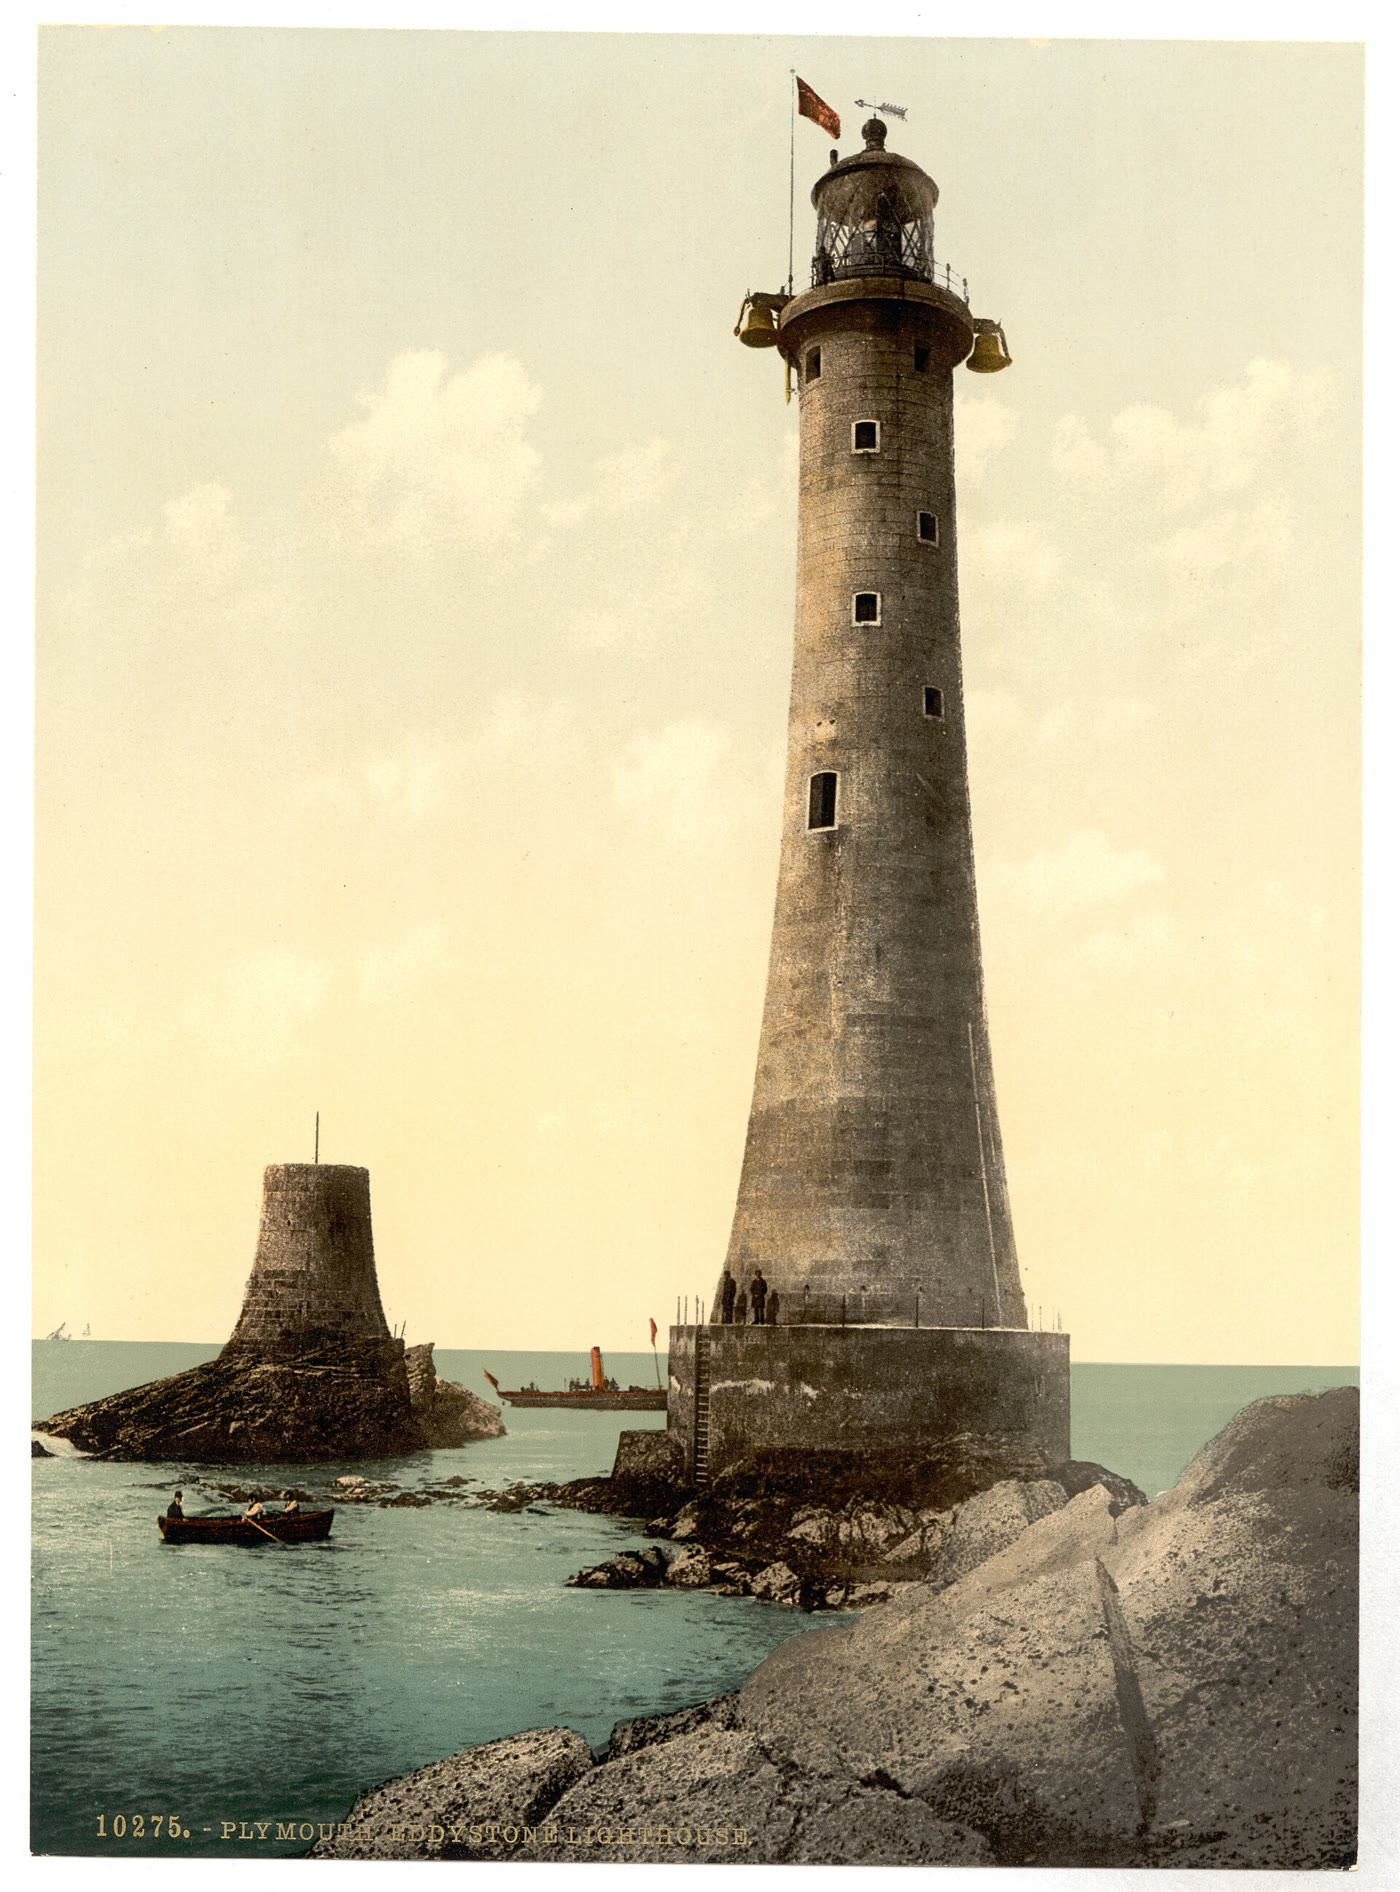
\includegraphics[width=0.34\linewidth]{images/book2/photos/g11-commons-eddystone-lighthouse.jpg}

{\small The Eddystone lighthouse off Plymouth, England, in a print of 1890--1900. On the left stands the stump of the tower of 1759 that it replaced.}
\end{omfigure}

\section{Overuse of a common resource}\label{sec:g11:public-goods-and-commons:open-access}

\begin{definition}[Tragedy of the commons]\label{def:g11:public-goods-and-commons:tragedy}
The \emph{tragedy of the commons}\index{tragedy of the commons} is the overuse of a \omterm{def:g11:public-goods-and-commons:private-good}{common resource} by users who each bear only part of the cost of their use.
\end{definition}

Take a fishing ground. The more boats fish it, the fewer fish each boat catches, because the stock is smaller. A boat owner who decides whether to join compares his
own catch with his cost; he ignores that his boat lowers every other boat's catch. That is a \omterm{def:g11:externalities:externality}{negative externality}, imposed by each boat on all the others.

\begin{model}{Open access to a common resource}
\assumes Anyone may enter; each boat's catch falls as the number of boats rises; boats are alike and cost the same.
\predicts Boats enter until the value of a boat's catch equals its cost: the fishery's rent (its revenue minus its cost) is dissipated, and beyond some fleet size
  the total catch falls as boats are added.
\tested Across more than 11\,000 fisheries from 1950 to 2003, those without catch shares collapsed about twice as often as those with them
  (Costello, Gaines and Lynham 2008, below). Consistent with it, though the 1972 El Niño also struck: Peru's fleet grew until the anchoveta collapsed in
  1972--73. The northern cod off Newfoundland fell to about 1\,\% of its former level, and in 1992 the government closed the fishery; more than
  35\,000 fishermen and plant workers lost their jobs.
% ledger: g11:costello2008
\breaks Where users are few, know each other, and enforce their own rules (field studies found long-lasting rules in Swiss and Japanese mountain villages,
  Spanish and Philippine irrigation and some fisheries; Ostrom 1990), and where rights to the catch are secure and can be traded.
\end{model}
% ledger: g11:anchoveta, g11:cod-1992, g11:ostrom1990

\begin{omfigure}
\begin{tikzpicture}[econ, x=0.072cm, y=0.28cm]
\draw[econ axes] (0,17.5) node[left, font=\small] {thousand kests} |- (105,0) node[below left=12pt and 0pt, font=\small] {boats $n$};
\draw[demand, domain=0:100, samples=60] plot (\x, {0.6*\x - 0.006*\x*\x});
\node[omDef, font=\scriptsize, above] at (50,15) {revenue $600n - 6n^2$};
\draw[supply] (0,0) -- (100,12) node[right, font=\scriptsize] {cost $120n$};
\draw[guide] (40,0) -- (40,14.4); \draw[guide] (80,0) -- (80,9.6);
\node[eqpoint] at (40,14.4) {}; \node[eqpoint] at (80,9.6) {};
\draw[<->, omThm, thick] (37,4.8) -- (37,14.4); \node[omThm, font=\scriptsize, left] at (37,9.6) {rent 9.6};
\foreach \y in {5,10,15} \draw (0,\y) -- (-1,\y) node[left, font=\footnotesize] {\y};
\node[below, font=\footnotesize] at (40,0) {40}; \node[below, font=\footnotesize] at (80,0) {80}; \node[below, font=\footnotesize] at (100,0) {100};
\end{tikzpicture}

{\small The Kestrian fishery of the weekend problem: a season's revenue and cost, in thousands of kests, against the number of boats. The rent, revenue minus cost, is largest at 40 boats.
Under open access boats keep entering until revenue equals cost, at 80 boats, where the rent is zero and the total catch is smaller.}
\end{omfigure}

\section{Answers and their record}\label{sec:g11:public-goods-and-commons:answers}

\begin{definition}[Individual transferable quota]\label{def:g11:public-goods-and-commons:itq}
An \emph{individual transferable quota}\index{individual transferable quota} is the right to catch a fixed share of a total allowed catch, which its holder may use,
lease or sell.
\end{definition}

The answers follow from the diagnosis. If the problem is that no one owns the resource, give someone a right to it: a property right over a pasture or a forest, or
a right to a share of the catch. A quota holder gains nothing by racing others for the fish, since his share is his, and the value of his quota rises when the stock
is well kept. Quotas are a tradable-permit market applied to a fishery: the total catch is capped, and the permits go to the boats that can use them at the least cost.
Where users are few and live together, their own rules, with monitors and graduated penalties, can do the same work without the state or a market.

\begin{omchart}{Fish caught by Iceland's and New Zealand's fleets, 1960--2022, in thousands of tonnes a year, times-ten scale. The dashed lines mark the year each
country made its fishing quotas transferable: New Zealand in 1986, Iceland in 1990.}{World Bank, World Development Indicators (capture fisheries production); dates:
reference sources in the ledger}
\begin{tikzpicture}
\begin{semilogyaxis}[omtime, width=0.84\linewidth, height=5.4cm, xmin=1960, xmax=2022, ymin=30, ymax=3000, ylabel={thousand tonnes},
  log ticks with fixed point, ytick={100,1000}, xtick={1960,1970,...,2020}]
\addplot[omDef, thick] table[x=year, y=ISL] {figdata/grade-11/07-public-goods-and-commons/out/itq.csv} node[pos=0.13, below=4pt, font=\scriptsize] {Iceland};
\addplot[omThm, thick] table[x=year, y=NZL] {figdata/grade-11/07-public-goods-and-commons/out/itq.csv} node[pos=0.13, above=3pt, font=\scriptsize] {New Zealand};
\addplot[black, dashed, ycomb, no markers] table[x=year, y=top] {figdata/grade-11/07-public-goods-and-commons/out/itq_dates.csv};
\end{semilogyaxis}
\end{tikzpicture}
\end{omchart}
% ledger: g11:itq-dates; figdata: itq_key

A chart of catches cannot show whether quotas worked: a falling catch may be a quota protecting a stock, or a stock in decline. The test needs many fisheries and
a measure of collapse. A study of more than 11\,000 fisheries from 1950 to 2003 found that nearly a third of those without catch shares had collapsed, and only about
half that share of those managed by catch shares. Quotas have their own record of trouble: who receives them at the start, and whether a few firms come to hold them
all, are questions the model does not settle.
% ledger: g11:costello2008

\begin{record}[The anchoveta collapse, 1972--73]
% ledger: g11:anchoveta; figdata: peru_key, peru (1960 3506)
Peru's catch rose from 3.5 million tonnes in 1960 to 12.5 million in 1970. In 1972 an El Niño stopped the rising
of cold, nutrient-rich water along the coast. Fish that had already been heavily caught found less food, and the catch fell to 4.7 million tonnes in 1972 and 2.3
million in 1973. The two causes cannot be fully separated, but a stock that has been fished down has less to fall back on when the sea turns against it.
\end{record}

International commons are harder still. The atmosphere, the open ocean and migrating fish stocks belong to no country, and no state can tax the others. An agreement
among countries to restrain their use is a contribution \omterm{def:g11:oligopoly-and-games:game}{game}: each country gains from the others' restraint and is tempted to free ride on it, and nothing forces it
to sign or keep its word.

\section{Exercises}

\begin{exercise}[$\star$]\label{exo:g11:public-goods-and-commons:1}
Classify as \omterm{def:g11:public-goods-and-commons:private-good}{private good}, \omterm{def:g11:public-goods-and-commons:private-good}{club good}, \omterm{def:g11:public-goods-and-commons:private-good}{common resource} or \omterm{def:g11:public-goods-and-commons:private-good}{public good}, and say why: a sandwich; fish in the open ocean; national defence; a film in a cinema.
\end{exercise}

\begin{exercise}[$\star$]\label{exo:g11:public-goods-and-commons:2}
Classify: a fireworks display seen from all over town; a paid swimming pool that is rarely full; groundwater pumped by farmers; a pair of shoes.
\end{exercise}

\begin{exercise}[$\star$]\label{exo:g11:public-goods-and-commons:3}
A road is free and empty at night and free and jammed at rush hour. Classify it in each case, and say how a toll would change the classification.
\end{exercise}

\begin{exercise}[$\star$]\label{exo:g11:public-goods-and-commons:4}
From the opening chart, read Peru's catch in 1970 and 1973 (in millions of tonnes, to one decimal) and compute the fall in percent.
\end{exercise}

\begin{exercise}[$\star$]\label{exo:g11:public-goods-and-commons:5}
In the opening chart, in which year did Peru's catch first pass 12 million tonnes again after 1973? How many years after the collapse was that?
\end{exercise}

\begin{exercise}[$\star\star$]\label{exo:g11:public-goods-and-commons:6}
In a lake, each boat catches $50 - n/2$ tonnes a season when $n$ boats fish. Fish sell at 2 dalens a tonne, and a boat costs 60 dalens a season. Under open access, how
many boats fish, and what is the total catch?
\end{exercise}

\begin{exercise}[$\star\star$]\label{exo:g11:public-goods-and-commons:7}
In \cref{exo:g11:public-goods-and-commons:6}, cheaper engines cut the cost of a boat to 40 dalens. Find the new open-access fleet and the total catch. Who gains from the
cheaper engines?
\end{exercise}

\begin{exercise}[$\star\star$]\label{exo:g11:public-goods-and-commons:8}
In \cref{exo:g11:public-goods-and-commons:6}, find the number of boats that maximises the lake's rent, the total catch, and the rent.
\end{exercise}

\begin{exercise}[$\star\star$]\label{exo:g11:public-goods-and-commons:9}
The lake's authority in \cref{exo:g11:public-goods-and-commons:6} issues transferable quotas for the efficient total catch. How many tonnes does it allow, and what
does the right to catch one tonne for one season lease for?
\end{exercise}

\begin{exercise}[$\star\star$]\label{exo:g11:public-goods-and-commons:10}
A swimming club costs 30\,000 dalens a year plus 20 dalens for each member. At a fee of 80 dalens a year, how many members must it have to cover its cost? Why can a
\omterm{def:g11:public-goods-and-commons:private-good}{club good} be sold, while a \omterm{def:g11:public-goods-and-commons:private-good}{public good} cannot?
\end{exercise}

\begin{exercise}[$\star\star$]\label{exo:g11:public-goods-and-commons:11}
From the chart of Iceland's and New Zealand's catches, read each country's catch in the year its quotas became transferable and in 2020. Do these numbers show that the
quotas worked? Explain.
\end{exercise}

\begin{exercise}[$\star\star\star$]\label{exo:g11:public-goods-and-commons:12}
What evidence would contradict the open-access model's prediction that a \omterm{def:g11:public-goods-and-commons:private-good}{common resource} is always overused? Use the field studies in the model box, and say which of the
model's assumptions they break.
\end{exercise}

\begin{exercise}[$\star\star\star$]\label{exo:g11:public-goods-and-commons:13}
$n$ players each hold 10 dalens and choose a contribution $g_i$ between 0 and 10; the total is multiplied by $m$, with $1 < m < n$, and shared equally. Show that giving
nothing is each player's dominant choice, and that all giving 10 leaves every player better off than all giving nothing.
\end{exercise}

\begin{exercise}[$\star\star\star$]\label{exo:g11:public-goods-and-commons:14}
Two countries each decide whether to cut emissions. Cutting costs the country that cuts 10; each cut brings a benefit of 6 to each country. Write the \omterm{def:g11:oligopoly-and-games:game}{payoff} table,
find the \omterm{def:g11:oligopoly-and-games:nash}{Nash equilibrium}, and show that it is a \omterm{def:g11:oligopoly-and-games:prisoners-dilemma}{prisoner's dilemma}. What would an agreement need to hold?
\end{exercise}

\begin{exercise}[$\star\star\star$]\label{exo:g11:public-goods-and-commons:15}
A one-tonne quota earns its holder a rent of 6 dalens a season, every season. At an interest rate of 5\,\% a season, what is the most a buyer would pay for the quota?
What happens to its price if the stock recovers and the rent rises to 8? If the authority announces that all quotas will be cancelled after one season?
\end{exercise}

\section{Problem: The Kestrian Fishery}

\begin{problem}[{Weekend problem --- open access, the efficient fleet and a quota market}]
\label{pb:g11:public-goods-and-commons:1}
In a bay of Kestria, each boat catches $100 - n$ tonnes of fish a season when $n$ boats fish. Fish sell at 6 kests a tonne, and running a boat for a season costs
120 kests. Anyone may fish.

\medskip
\noindent\textbf{Part I --- Open access.}
\begin{enumerate}
\item Write the value of one boat's catch and the bay's total revenue as functions of $n$.
\item How many boats fish under open access?
\item Find each boat's catch, the total catch and the rent at that fleet.
\item Show that a boat that joins lowers every other boat's catch. By how much does the 80th boat cut the others' total catch?
\item Explain why each owner ignores that loss.
\end{enumerate}

\medskip
\noindent\textbf{Part II --- The efficient fleet.}
\begin{enumerate}[resume]
\item Write the rent $R(n)$, revenue minus cost, and find the $n$ that maximises it.
\item Find each boat's catch, the total catch and the rent at that fleet.
\item Find the fleet that maximises the total catch, and the catch there.
\item Compare the three fleets: which catches most, which earns most?
\item How much rent does open access dissipate each season?
\end{enumerate}

\medskip
\noindent\textbf{Part III --- Quotas.}
\begin{enumerate}[resume]
\item The authority caps the season's catch at the efficient total and issues one-tonne transferable quotas. How many quotas does it issue?
\item Compute the rent per tonne at the efficient fleet: price minus the cost of catching a tonne.
\item Explain why a quota for one tonne and one season leases at that rent.
\item A quota gives the right to one tonne every season for ever. At an interest rate of 5\,\% a season, what does it sell for?
\item Why would an owner who holds quotas want the stock kept healthy?
\end{enumerate}

\medskip
\noindent\textbf{Part IV --- Limits.}
\begin{enumerate}[resume]
\item The authority gives the quotas free to the 80 boats fishing on the day of the reform, equally. How many tonnes does each receive, and what is its quota worth?
\item After trading, 40 boats fish. What do the 40 boats that leave receive, and from whom?
\item If the authority sets the total at 2100 tonnes by mistake, how many boats fish, and what is the rent?
\item Name one cost of quotas that the model leaves out.
\item State the result of the problem: the rent dissipated under open access and the price of a one-tonne quota.
\end{enumerate}
\end{problem}
